\documentclass[11pt,a4paper]{article}

\usepackage{fontspec}
\usepackage[margin=2.5cm]{geometry}
\usepackage{graphicx}
\usepackage{longtable}
\usepackage{booktabs}
\usepackage{array}
\usepackage[most]{tcolorbox}
\usepackage{overpic}
\usepackage{hyperref}
\usepackage{titlesec}
\usepackage{enumitem}
\usepackage{xcolor}

\definecolor{easyamber}{HTML}{B98530}
\definecolor{easytext}{HTML}{1D2126}

\hypersetup{
  colorlinks=true,
  linkcolor=easyamber,
  urlcolor=easyamber,
  pdftitle={EASy68K Web -- User Manual},
  pdfauthor={Antoni Burguera}
}

\titleformat{\section}{\normalfont\Large\bfseries\color{easyamber}}{\thesection}{1em}{}
\titleformat{\subsection}{\normalfont\large\bfseries}{\thesubsection}{1em}{}

\setlength{\parskip}{0.5em}
\setlength{\parindent}{0pt}

\graphicspath{{images/}}

\title{\textbf{EASy68K Web}\\[0.3cm]\Large User Manual}
\author{Antoni Burguera\\\small{Universitat de les Illes Balears}}
\date{\today}

\begin{document}

\maketitle

\begin{tcolorbox}[colback=gray!5!white,colframe=gray!60!black,title=About this manual]
This manual documents the browser-based EASy68K Web application: what each
button and panel does, and what you need to know about its virtual
file system before trusting it with real work. It does not document the
Motorola 68000 instruction set or 68000 assembly programming in general --
only this specific application's own user interface and its TRAP \#15
extensions (the latter fully documented in the companion
\emph{TRAP \#15 Reference}, \texttt{trap15\_reference.pdf}). This same
content, kept in sync, is also available inside the application itself
through its own \textbf{Help} button. For anything about EASy68K itself,
the 68000 instruction set, or assembly-language programming in general
that this manual doesn't cover, see EASy68K's own official documentation
at \url{http://www.easy68k.com/}.
\end{tcolorbox}

\tableofcontents
\vspace{1cm}

\section{Overview}

\subsection*{What this is}
This is a browser port of EASy68K — a 68000 assembler, simulator, and IDE — built from the real original C++ source, compiled to run in your browser. \textbf{Nothing you do here is ever uploaded anywhere}; the assembler, the simulator, and every file you work with all run entirely on your own machine, inside this page.


\begin{figure}[h]
  \centering
  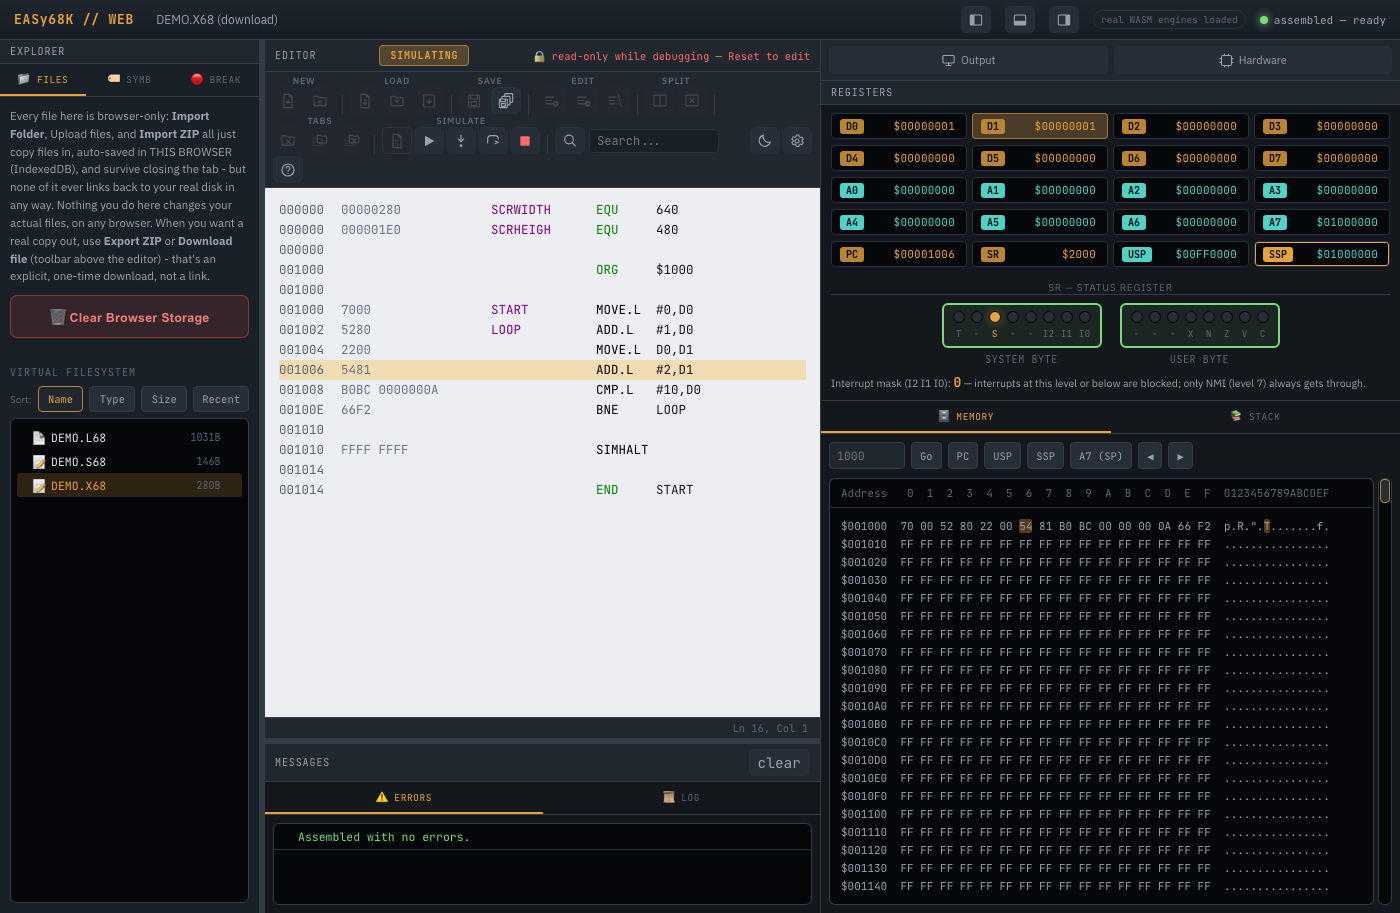
\includegraphics[width=\textwidth]{overview_debugging.png}
  \caption{EASy68K Web while debugging a program: the code listing (center) with the current instruction highlighted, the register/memory panel (right), the file explorer (left), and the assembler messages (bottom).}
\end{figure}

\clearpage
\section{Getting started}

Open \texttt{dist/easy68k-web.html} directly in any modern browser -- no
installation, no server, no account. Everything, including the assembler
and the simulator, runs locally on your own machine.

\begin{enumerate}[label=\arabic*.]
  \item Create a new file (toolbar \textbf{New} group) or import an existing project.
  \item Write or paste your 68000 assembly source.
  \item Click \textbf{Assemble}. If it succeeds, the view switches to the simulator.
  \item Click \textbf{Run}, or \textbf{Step} through the program one instruction at a time.
  \item Click \textbf{Reset} to go back to editing.
\end{enumerate}

\section{Layout overview}

The application window is divided into four regions, all visible in
Figure~\ref{fig:overview}:

\begin{itemize}
  \item \textbf{Left -- Explorer}: the virtual file tree.
  \item \textbf{Center -- Editor / Simulator}: the source code editor while editing, or the assembled listing while simulating.
  \item \textbf{Right -- Registers, Memory \& Stack}: the debugger panels.
  \item \textbf{Bottom -- Messages}: assembler errors/warnings and the runtime log.
\end{itemize}

\begin{figure}[h]
  \centering
  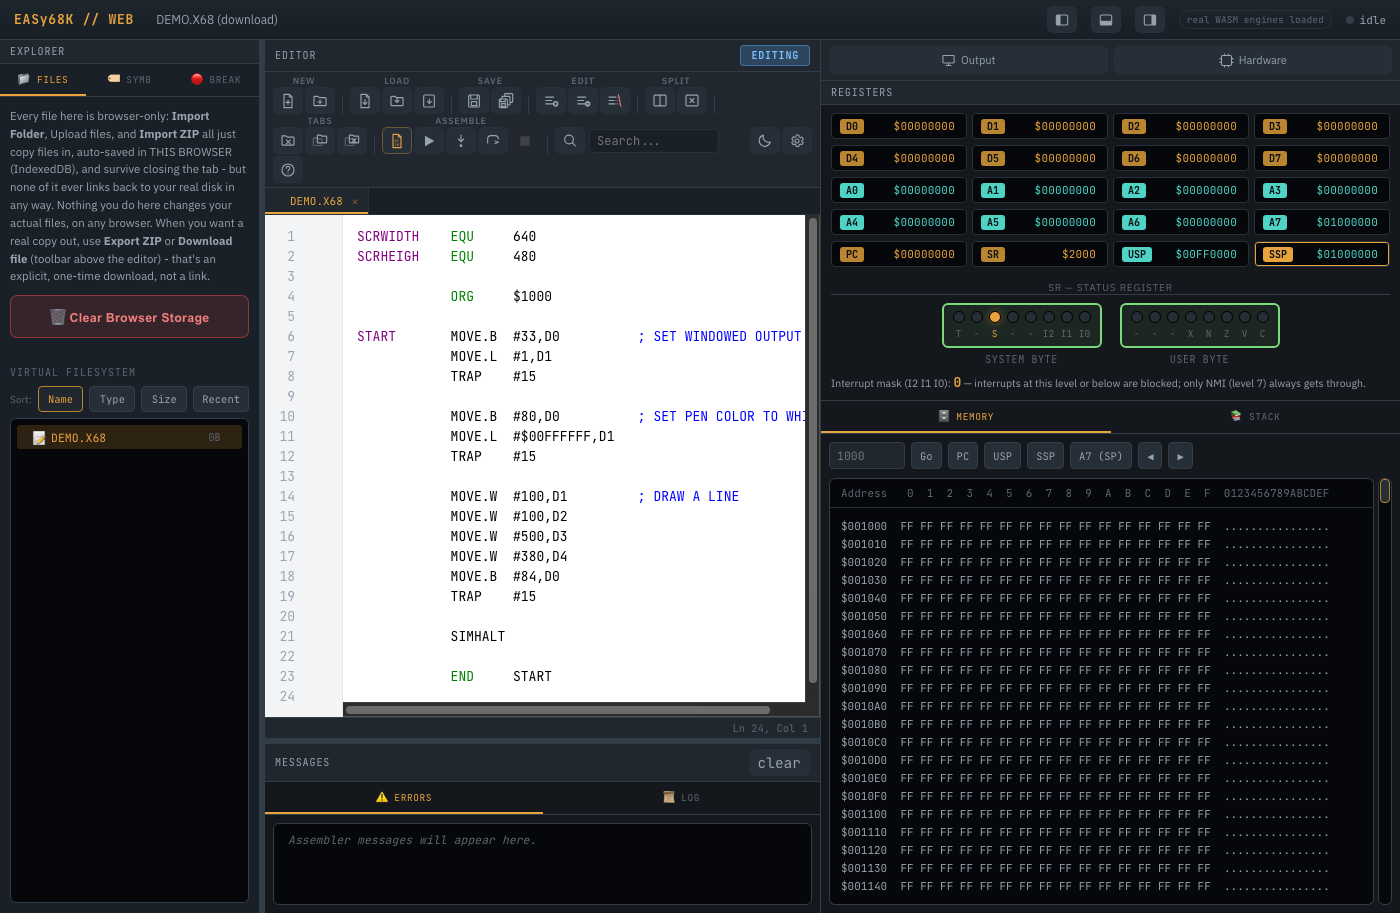
\includegraphics[width=\textwidth]{overview_editing.png}
  \caption{The four regions of the interface, shown here in Editing mode with no file open.}
  \label{fig:overview}
\end{figure}

\clearpage
\subsection*{Top bar: panel visibility}
The bar along the very top (with the "EASy68K // WEB" brand and the engine/status indicators) has three \textbf{panel-visibility} toggles, right before those indicators: they hide/show the left (Explorer), right (Registers/Memory/Stack), and bottom (Messages) panels — each icon shows which panel it controls (a small rectangle with that side highlighted) and dims once that panel is hidden. Hiding a panel lets the editor expand to fill the freed space — handy on a small screen (a laptop) where you want to focus on just the code for a while. Every hidden panel can always be brought back with the same button; these buttons live in the top bar specifically (not inside the panels themselves) so they stay reachable even while their panel is hidden. Which panels are visible is remembered across reloads.

A separate \textbf{(moon)/(sun) theme toggle} (dark by default; your choice is remembered too) lives in the editor's own toolbar, next to the search box and the Settings/Help icons.


\begin{figure}[h]
  \centering
  \begin{overpic}[width=0.5\textwidth]{topbar_closeup.png}
    \put(6,-8){\small 1}
    \put(24,-8){\small 2}
    \put(42,-8){\small 3}
  \end{overpic}
  \caption{The three panel-visibility toggles in the top bar: (1) left/Explorer, (2) bottom/Messages, (3) right/Registers-Memory-Stack.}
\end{figure}

\subsection*{The two modes: Editing and Simulating}
The app is always in one of two modes, shown by the badge next to the "Editor" title:

\begin{itemize}
\item \textbf{EDITING} — write and manage source files. The toolbar's last group is labeled \textbf{ASSEMBLE}; only its \textbf{Assemble} button is active.
\item \textbf{SIMULATING} — after a successful Assemble, the view switches to a read-only listing of your program (source and machine code merged, matching the real assembler's \texttt{.L68} listing) and the same toolbar group relabels to \textbf{SIMULATE}, enabling \textbf{Run}, \textbf{Step}, \textbf{Step Over}, and \textbf{Reset}. The editor itself becomes read-only while simulating ((lock) shown in the title bar) — press \textbf{Reset} to return to editing.
\end{itemize}
\begin{tcolorbox}[colback=blue!5!white,colframe=blue!60!black,title=Note]
\textbf{Breakpoints only exist during simulation.} Click a line number in the listing to toggle one; Run stops when the PC reaches it. They're cleared every time you Reset, so a breakpoint never ends up pointing at the wrong line after you've since edited the file.
\end{tcolorbox}

\clearpage
\subsection*{Editor toolbar}
Grouped left to right, above the source editor:

\begin{longtable}{@{}p{3.0cm}p{3.4cm}p{7.8cm}@{}}
\toprule
\textbf{Group} & \textbf{Button} & \textbf{Does} \\
\midrule
\endfirsthead
\toprule
\textbf{Group} & \textbf{Button} & \textbf{Does} \\
\midrule
\endhead
New & New file / New folder & Creates an empty file (from a small default template, optional) or folder in the virtual file system, inside whichever folder is currently selected in the Files panel. \\
Load & Import file… & Adds one file to the virtual file system. \\
 & Import folder… & Copies an entire local folder in, preserving its structure. If any project is already open, this \textbf{replaces the whole virtual file system}, not just files with matching names - you're asked to confirm first, with an option to download a backup ZIP of what's about to be deleted. \\
 & Import ZIP… & Same as Import Folder (including the same whole-project replace-and-confirm behavior), from a \texttt{.zip} archive. \\
Save & Download file & Downloads the current file to your real disk. Always a fresh, explicit download (\texttt{Ctrl/Cmd+S}) — never a silent "save". \\
 & Export ZIP & Downloads every file in the virtual file system as one \texttt{.zip} archive. \\
Edit & Comment out / Uncomment & Toggles a leading \texttt{*} comment marker on every selected line. \\
 & Remove trailing spaces & Strips trailing spaces/tabs from every line of the current file (the whole file, not just a selection) - purely cosmetic, has no effect on assembling. \\
Split & Split editor / Close all splits & Opens a second editor pane side by side (so you can view/edit two files at once) or collapses back to one. \\
Tabs & Close current tab & Closes the active file tab. \\
 & Close other tabs & Closes every tab except the active one. \\
 & Close all tabs & Closes every open tab. \\
Assemble/Simulate & Assemble & Builds the current file with the real EASy68K assembler. On success, switches to Simulating; on failure, opens the Assembly Failed dialog listing every error. \\
 & Run / Pause & Runs continuously until it halts, hits a breakpoint, or you press Pause. \\
 & Step & Executes exactly one instruction. \\
 & Step Over & Like Step, but a \texttt{BSR}/\texttt{JSR} call runs to completion in one go rather than single-stepping into the subroutine. \\
 & Reset & Stops simulation and returns to Editing. Also the only way breakpoints and simulator-only state get cleared. \\
\bottomrule
\end{longtable}
To the right of the groups: a \textbf{search} box (Enter to find/advance), \textbf{Editor settings} (font, size, tab width, column mark), and this \textbf{Help} button.

A thin amber \textbf{column-mark line} runs down the editor at a fixed column (80 by default) - a visual guide only, it has no effect on assembling. Its column is editable in Settings. A status bar along the bottom of the editor shows the cursor's current \textbf{line and column} (\texttt{Ln, Col}), updated as you type, click, or move the caret with the keyboard.


\begin{figure}[h]
  \centering
  \begin{overpic}[width=\textwidth]{toolbar_closeup.png}
    \put(1,-6){\small 1}
    \put(16,-6){\small 2}
    \put(29,-6){\small 3}
    \put(41,-6){\small 4}
    \put(53,-6){\small 5}
    \put(66,-6){\small 6}
  \end{overpic}
  \vspace{0.3cm}
  \caption{Editor toolbar groups: (1) New, (2) Load, (3) Save, (4) Edit, (5) Split, (6) Tabs/Assemble-Simulate row below (not numbered individually -- see table above). The moon/sun icon on the far right is the theme toggle; the gear icon opens Settings.}
\end{figure}

\clearpage
\section{The Files panel and the virtual file system}

\begin{figure}[h]
  \centering
  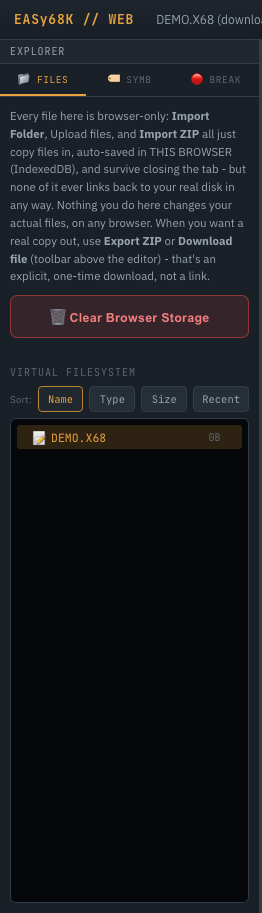
\includegraphics[width=0.35\textwidth]{left_panel_closeup.png}
  \caption{The Explorer panel: the Files tab, its virtual filesystem tree, and the ``Clear Browser Storage'' action.}
\end{figure}

\subsection*{Files panel \& the virtual file system}
The left-hand \textbf{Files} tab is a small file tree with its own right-click context menu (New File/Folder, Upload files/ZIP, Rename, Cut, Copy, Paste, Delete) and drag-and-drop for moving or copying entries between folders. Files can also be dragged in directly from your desktop.

\begin{tcolorbox}[colback=red!5!white,colframe=red!60!black,title=Warning]
\textbf{Nothing here is ever linked to your real disk.} Import Folder, Upload files, and Import ZIP all just \textit{copy} files into the browser — they're auto-saved locally (IndexedDB) and survive closing the tab or reloading the page, but editing them here never changes your real files, on any browser, and nothing you import is ever sent anywhere. To get a real copy back out, use \textbf{Export ZIP} or \textbf{Download file} — an explicit, one-time download, not an ongoing link.\par \par 
      This storage is \textbf{private to this one browser} (not synced across browsers, devices, or even a regular vs. private/incognito window in the same browser), and it can be erased not only by this app's own \textbf{Clear Browser Storage} button (which is permanent and cannot be undone) but also by clearing site data/cookies for this page from your browser's own settings. If a project matters, keep a real copy on disk via Export ZIP — don't rely on browser storage as your only copy.
    
\end{tcolorbox}

\clearpage
\section{Registers, Memory and Stack}

\subsection*{Registers, Memory \& Stack (right column)}
\begin{itemize}
\item \textbf{Registers} — D0-D7, A0-A7, PC, SR, USP, SSP, and the individual SR flag/interrupt-mask bits. Values are editable directly (click and type) while simulating.
\item \textbf{Memory} — a scrollable hex/ASCII dump. Jump to an address, or straight to PC/USP/SSP/A7. Click a byte to start "type-through" editing (2 hex digits, or 1 ASCII character, auto-advancing to the next byte) — an invalid entry briefly flashes red and reverts rather than silently failing.
\item \textbf{Stack} — three independent stack views at once, each pointed at any address register or at the User/Supervisor stack pointer specifically.
\end{itemize}

\begin{figure}[h]
  \centering
  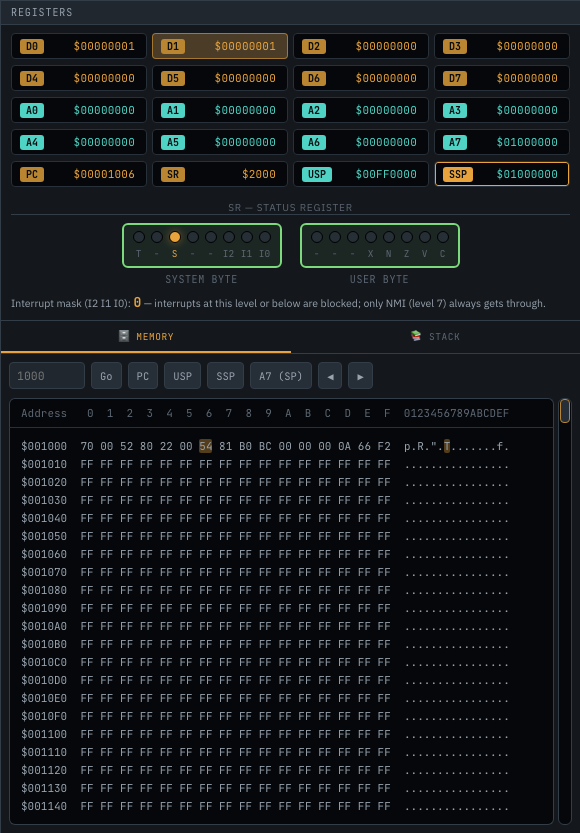
\includegraphics[width=0.5\textwidth]{right_panel_closeup.png}
  \caption{The Registers panel, the Status Register bit display, and the Memory hex/ASCII dump.}
\end{figure}

\clearpage
\subsection*{Output window}
Opened with the \textbf{Output} button (right toolbar). This is where your program's TRAP \#15 graphics and text output actually draws, at whatever resolution the program requests (640×480 by default). It's a real floating window: draggable, resizable, and independently maximizable to fullscreen (Esc, or its own restore button, to exit) — \textbf{Reset to actual size} snaps it back to exact 1:1 pixel scale.


\begin{figure}[h]
  \centering
  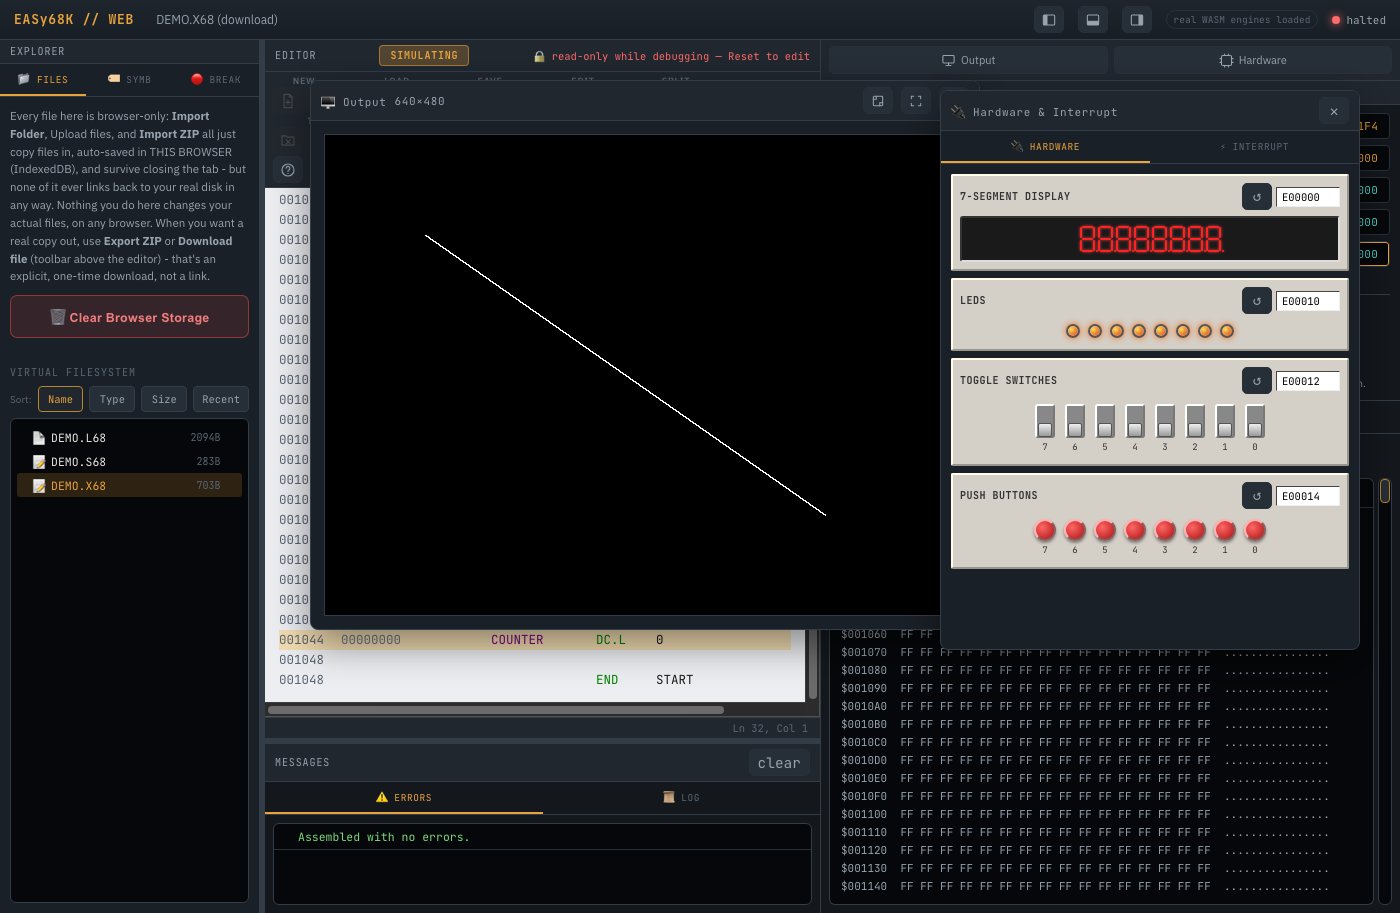
\includegraphics[width=0.7\textwidth]{overview_windows.png}
  \caption{The Output window (a program's TRAP \#15 graphics/text) and the Hardware \& Interrupt window, both open side by side.}
\end{figure}

\subsection*{Hardware \& Interrupt window}
Opened with the \textbf{Hardware} button. The \textbf{Hardware} tab shows the memory-mapped 7-segment display, LEDs, toggle switches, and push buttons a program can read/write like real peripherals — each device's mapped address is editable (with a one-click reset to its default). The \textbf{Interrupt} tab lets you fire IRQ levels 1-7 by hand, including an auto-repeat timer per level, to test a program's own interrupt handlers without needing real hardware.

\begin{tcolorbox}[colback=blue!5!white,colframe=blue!60!black,title=Note]
An interrupt only actually fires if its level is above SR's current interrupt-priority mask (real 68000 behavior, not a bug) — a masked IRQ button press is logged as masked rather than silently doing nothing.
\end{tcolorbox}

\clearpage
\subsection*{Settings}
The gear icon opens editor font/size/tab-width/column-mark preferences and one simulator option: which interrupt mask a run starts with (EASy68K's own convention of starting fully open, vs. real 68000 hardware's fully-masked reset state).

\begin{tcolorbox}[colback=blue!5!white,colframe=blue!60!black,title=Note]
This guide covers \textbf{this web port's own interface} — its panels, buttons, and windows. It does not teach the Motorola 68000 instruction set, assembly-language programming in general, or every assembler directive. For that, and for anything about EASy68K itself this guide doesn't go into, see EASy68K's own official documentation at \href{http://www.easy68k.com/}{easy68k.com}.
\end{tcolorbox}

\begin{figure}[h]
  \centering
  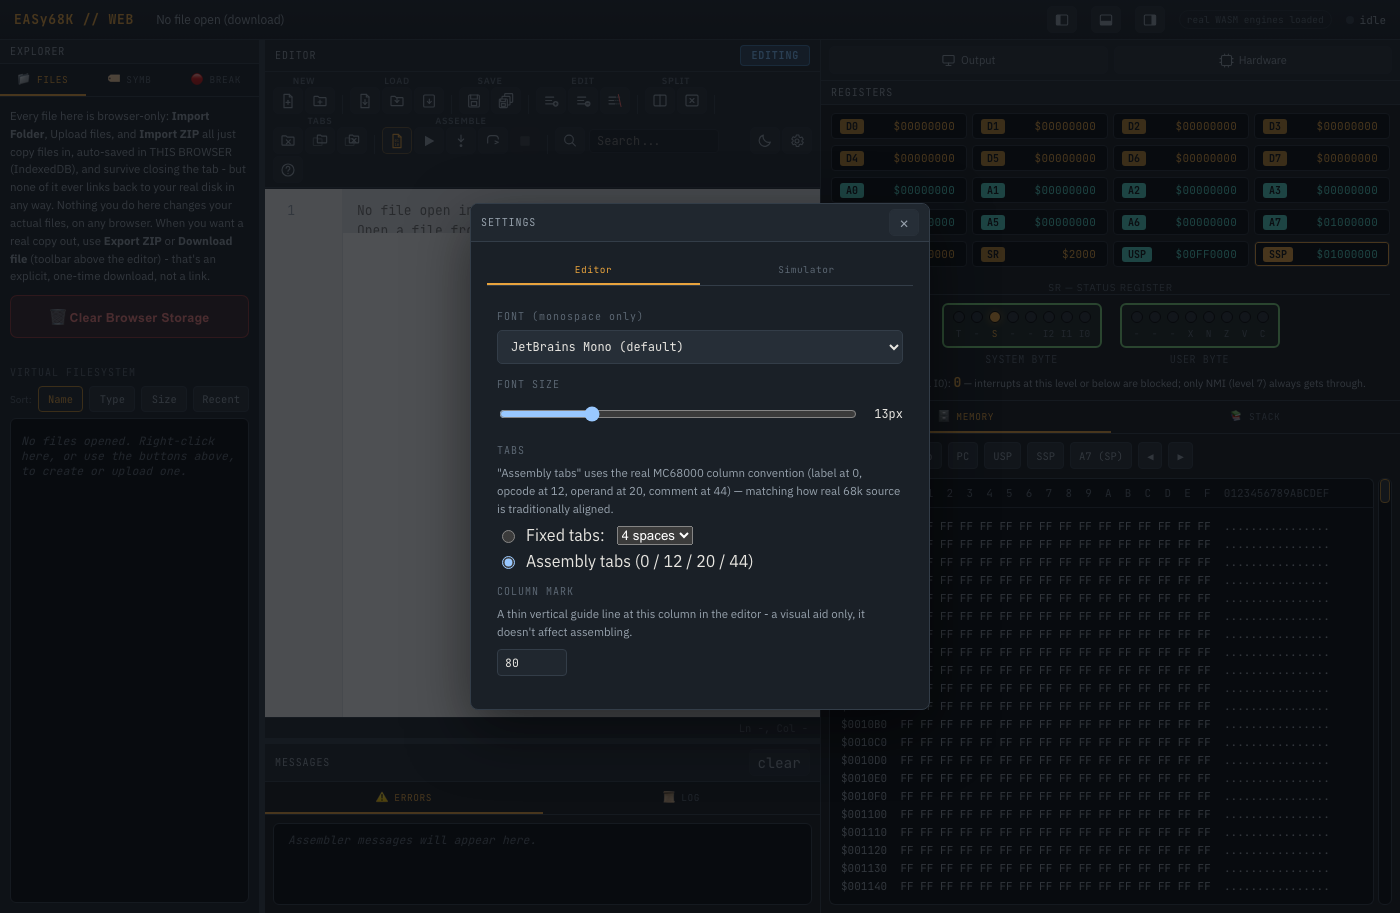
\includegraphics[width=0.7\textwidth]{settings_modal.png}
  \caption{The Settings dialog: editor font/size/tabs/column-mark preferences and the simulator's initial interrupt-mask option.}
\end{figure}

\clearpage
\section{In-app Help}

Every topic in this manual is also available inside the application
itself, always up to date with whichever version of the app you are
running: click the \textbf{Help} button (the question-mark icon, next to
Settings) to open it, side by side with your own work.

\begin{figure}[h]
  \centering
  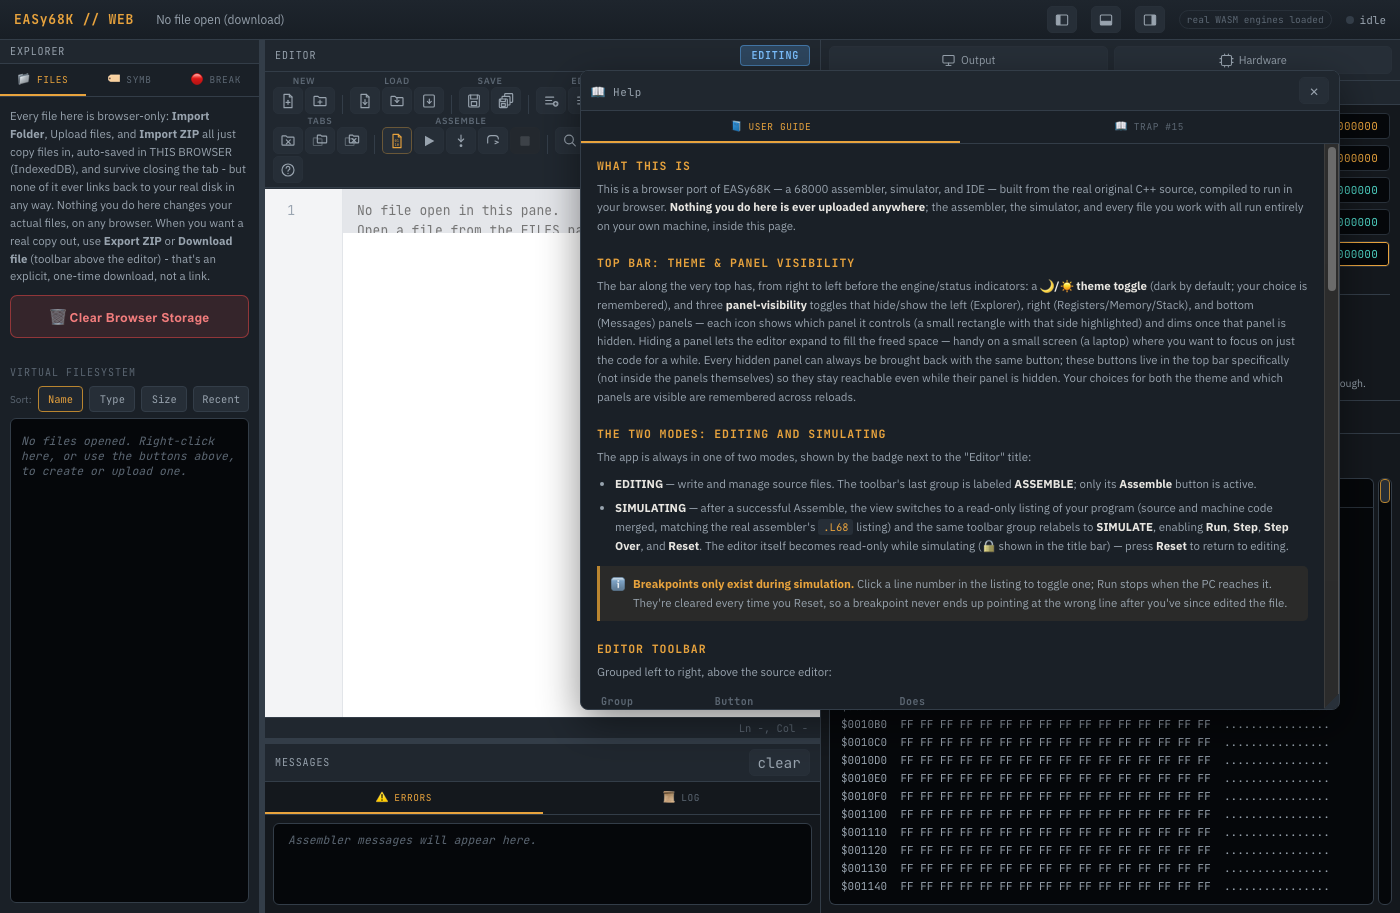
\includegraphics[width=\textwidth]{help_userguide.png}
  \caption{The in-app Help window, User Guide tab -- the same content as this manual, plus the full TRAP \#15 reference in its own tab.}
\end{figure}

\vspace{1cm}
\begin{tcolorbox}[colback=gray!5!white,colframe=gray!60!black,title=See also]
For the complete, task-by-task TRAP \#15 reference (every parameter,
every register, fully documented), see the companion document
\emph{EASy68K Web -- TRAP \#15 Reference} (\texttt{trap15\_reference.pdf}).
\end{tcolorbox}

\end{document}
